\chapter{Implementation of Intelligent Traffic Management System}

This section outlines how the proposed design is translated into working code, hardware integration, and deployment setup. We detail the microcontroller wiring, sensor programming, and dashboard connection.

\section{Contents of this Section}
\begin{enumerate}
\item Sensor Hardware Integration
\item YOLOv5 Model Deployment
\item Arduino + ESP8266 Firmware
\item Web-Based Dashboard Interface
\end{enumerate}

\subsection{Hardware Implementation}

The hardware setup forms the backbone of the Vehicle Congestion and Control System, enabling real-time data collection and physical signal control. Each traffic junction is equipped with the following components to ensure accurate detection and efficient traffic management:

\begin{itemize}
    \item \textbf{IR Sensors:} Deployed near the stop lines to detect the presence of vehicles at static positions. These are essential for identifying waiting vehicles when the signal is red.
    
    \item \textbf{Ultrasonic Sensors:} Installed along the lanes to measure the distance of queued vehicles. This helps estimate the length of vehicle queues and determine congestion levels dynamically.
    
    \item \textbf{Camera Module:} Mounted at a suitable height to capture live traffic footage. These video feeds are used for vehicle detection and classification using the YOLOv5 model at the edge level.
    
    \item \textbf{Arduino Mega:} Acts as the central controller for signal management. It receives inputs from sensors, executes signal control logic, and interfaces with traffic lights accordingly.
    
    \item \textbf{ESP8266 Wi-Fi Module:} Provides wireless communication between the Arduino and backend server or edge processing units for data transfer and control signals.
    
    \item \textbf{Power Supply and Connectors:} Ensures continuous and stable power delivery to all hardware components deployed at the junction.
\end{itemize}

\vspace{0.3cm}

The hardware units are housed in weather-resistant enclosures for outdoor deployment and are modular to simplify maintenance and upgrades. The interaction among these components allows for automated traffic monitoring, adaptive signal control, and support for emergency vehicle prioritization, laying a solid foundation for a smart traffic management system.


\subsection{Software Integration}

In our project titled \textbf{Vehicle Congestion and Control System}, software integration plays a vital role in linking sensor data, machine learning models, and real-time web-based control logic into a cohesive prototype. The components interact across multiple layers as outlined below:

\begin{itemize}
    \item \textbf{Sensor Layer:} Infrared (IR) and Ultrasonic sensors are deployed to detect vehicle presence and monitor congestion levels at intersections.
    
    \item \textbf{Processing Layer:} An Arduino Mega in conjunction with ESP8266 modules collects data from sensors and transmits it wirelessly to the local processing unit.
    
    \item \textbf{Intelligence Layer:} A YOLOv5 model processes real-time traffic video feeds to detect and classify vehicles. Python scripts utilizing OpenCV and the YOLOv8 architecture are executed on an edge device such as Jetson Nano or Raspberry Pi.
    
    \item \textbf{Communication Layer:} Traffic data is transmitted via MQTT or HTTP to a Flask-based backend.
    
    \item \textbf{Control Layer:} The backend dynamically adjusts signal timings based on live congestion metrics and detects emergency vehicles to prioritize signal changes.
    
    \item \textbf{Web Layer:} A web dashboard built using HTML, CSS, and JavaScript displays real-time traffic status and control logic results. 
\end{itemize}

\vspace{0.3cm}

\textbf{Technologies Used:}
\begin{itemize}
    \item \textbf{Sensors and Software:} Python, OpenCV, YOLOv8, Arduino IDE, MQTT/HTTP protocols.
    \item \textbf{Web Technologies:} Flask or Django (backend), HTML/CSS/JS (frontend), data training and testing with Roboflow.
\end{itemize}

\vspace{0.3cm}

\textbf{Functional Highlights:}
\begin{itemize}
    \item Vehicle detection and classification using YOLOv5 from live video streams.
    \item Basic dashboard UI implemented with real-time status display.
    \item Signal control logic successfully simulated based on congestion patterns and sensor input.
\end{itemize}

\vspace{0.5cm}

This section illustrates the end-to-end integration of software with hardware layers, forming a complete and operational prototype. The following section presents the simulation results under various traffic scenarios and evaluates system responsiveness.
\begin{figure}[H]
\centering
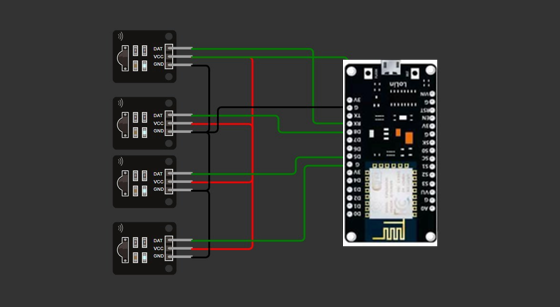
\includegraphics[width=0.65\textwidth]{Figures/ir.png}
\caption{Integration of multiple IR sensors with ESP8266 for real-time vehicle detection at signal junctions.}
\label{fig:ir-integration}
\end{figure}

\begin{figure}[H]
\centering
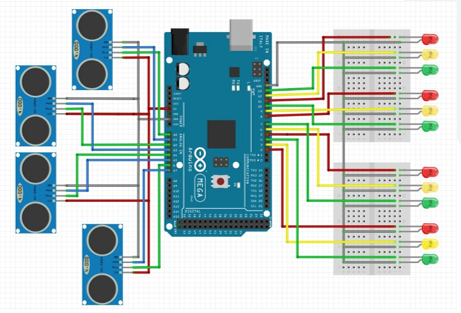
\includegraphics[width=0.75\textwidth]{Figures/us.png}
\caption{Ultrasonic sensors connected to Arduino Mega to monitor vehicle queue length and control traffic lights dynamically.}
\label{fig:us-integration}
\end{figure}

\vspace{0.5cm}

These figures illustrate the actual hardware implementation of the system. The first image demonstrates the IR sensor array interfaced with the ESP8266 module, which transmits vehicle presence data to the central controller. The second image shows the ultrasonic sensor layout connected to an Arduino Mega, which also drives the traffic light LEDs based on real-time congestion data. Together, these setups form the foundation of our intelligent traffic management prototype.


\vspace{0.5cm}